\documentclass[a4paper,10pt]{article}

\setlength\parindent{0pt}

\usepackage[utf8x]{inputenc} %soll utf8 als code verwenden
\PrerenderUnicode{äöüÄÖÜß} % umlaute gehen nun auch

\usepackage[ngerman]{babel} % deutsche Bezeichnungen

\usepackage{amssymb} % mathe symbole
\usepackage{amsmath} % mathe formeln
\usepackage{amsthm} % mathe theoreme
\usepackage{graphicx} % Darstellung von Bildern

\usepackage{pstricks}

% - Times, Helvetica, Courier (Word Standard...)
\usepackage{mathptmx}
\usepackage[scaled=.90]{helvet}
\usepackage{courier}
\usepackage{listings}

\newtheorem{lemma}{Lemma}

\begin{document}
\begin{lemma}
	Für jeden $U_2$ Schaltkreis $\beta$, gibt es einen äquivalnten Schaltkreis, welcher höchstens
	2 mal so groß ist wie $\beta$, in dem nur NOT-Gatter nur bei den Variablen benutzt werden.
\end{lemma}

Bei einem $U_2$ Schaltkreis handelt es sich um einen Schaltkreis bei dem nur die Gatter AND, OR und NOT mit 2 Eingängen verwendet werden.\\

Als erstes werden die Gatter topologisch sortiert. Also Gatter die andere Gatter an ihren Eingängen haben kommen nach diesen.\\
Nun beginnen wir mit dem obersten Gatter. Sollte dessen Ausgang verneint sein, so wenden wir darauf die Regel von deMorgan\footnote{$\overline{a\land{}b}=\overline{a}\lor\overline{b}$ Analog für OR} an.\\
Sollten die Ausgänge verneint sein so verschieben wir diese Verneinung auf die Ausgänge der vorhergehenden Gatter, wobei sich doppelte Verneinungen Aufheben.\\
Dies wird wiederholt für alle vorhergehenden Gatter.\\
Für den Fall, dass ein Gatter negiert und nicht negiert verwendet wird, wird dieses Gatter verdoppelt.\\
\qed{}

Um das zu verdeutlichen nehmen wir einen beispiel Schaltkreis: \\

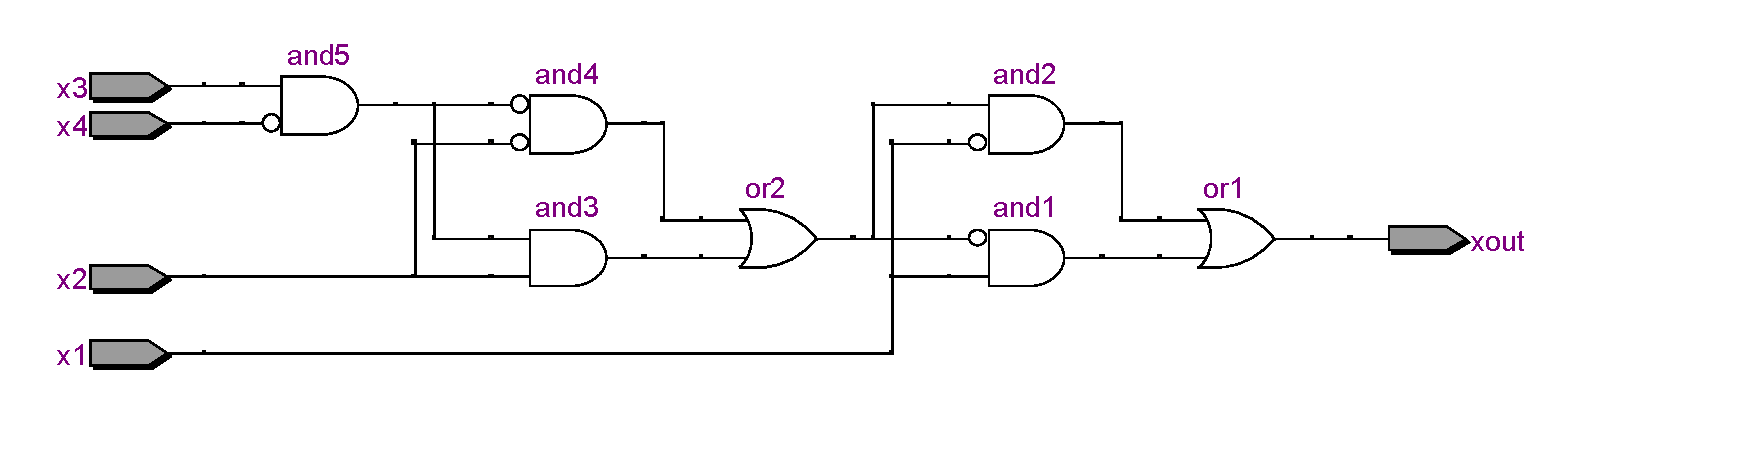
\includegraphics[scale=0.50]{images/ursk.pdf}

Dieser Schaltkreis ist um $U_2$ so wie es das Lemma bereits verlangt.
Es hat eine $C(s) = 7$ dem zu folge sollte der neue Schaltkreis maximal eine von $14$ haben.
Zu erst stellen wir zu jedem Input auch sein Inverses bereit und von oben nach Unten (top down) stellen wir nun
f\"ur jedes Gatter auch sein Inverses nach den Regeln von DeMorgan zu verf\"ugung.
Bei diesem Schritt kann es dazu kommen das wir zwei \"aquivalente Teilschaltkreise bekommen die wir zusammen f\"ugen k\"onnen. \\

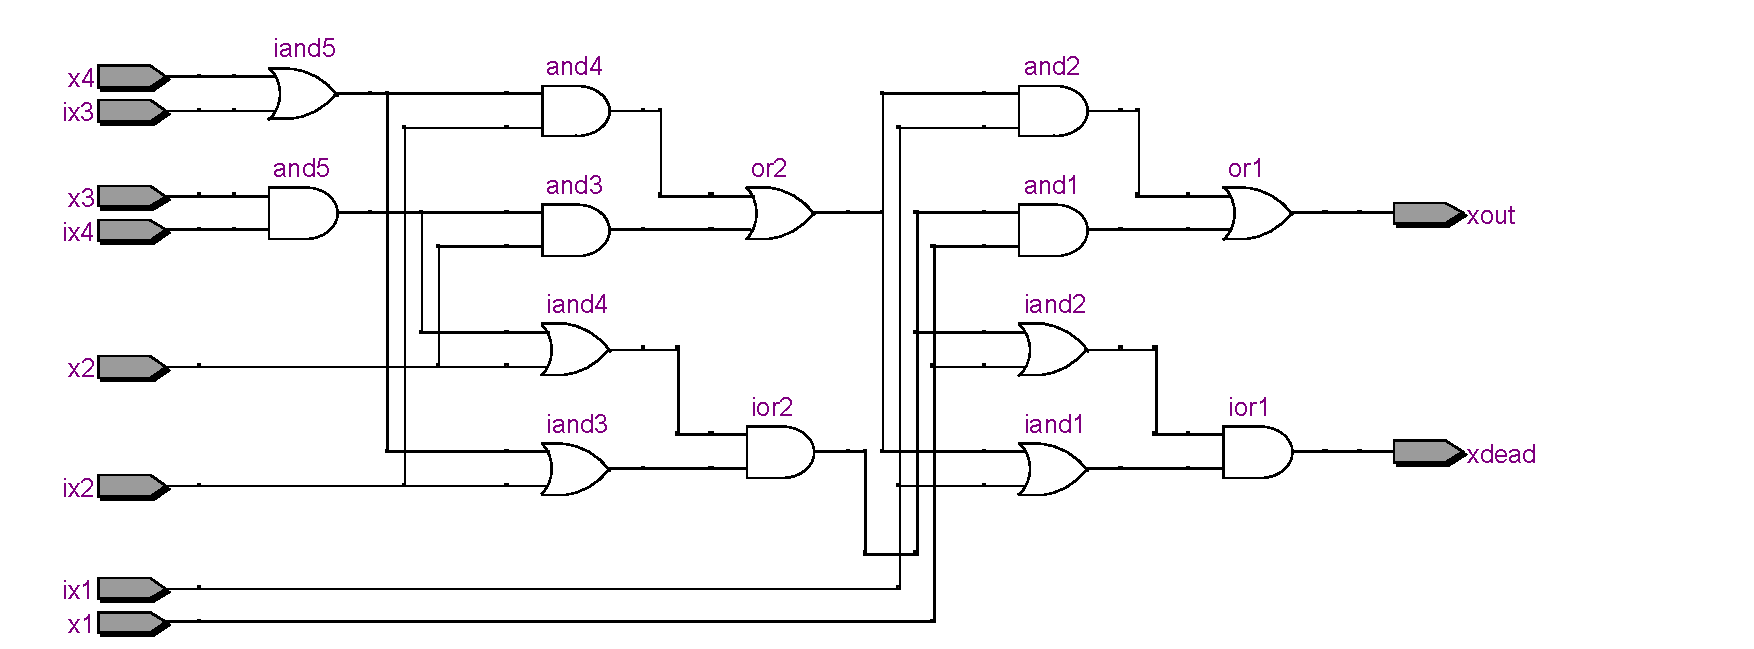
\includegraphics[scale=0.50]{images/zwisk.pdf}

Dieser neue Schaltkreis hat nun eine Komplexit\"at von $14$, also h\"alt er sich an das Lemma. Die Not-Gatter sind auch alle verschwunden und werden nun \"uber
die Inversen Inputs realisiert. Zum Schluss k\"onnen wir noch \glqq M\"ull\grqq entfernen. Also tote Gatter die wir nicht ben\"otigen da ihre Signale ins Nirvana verschwinden.\\

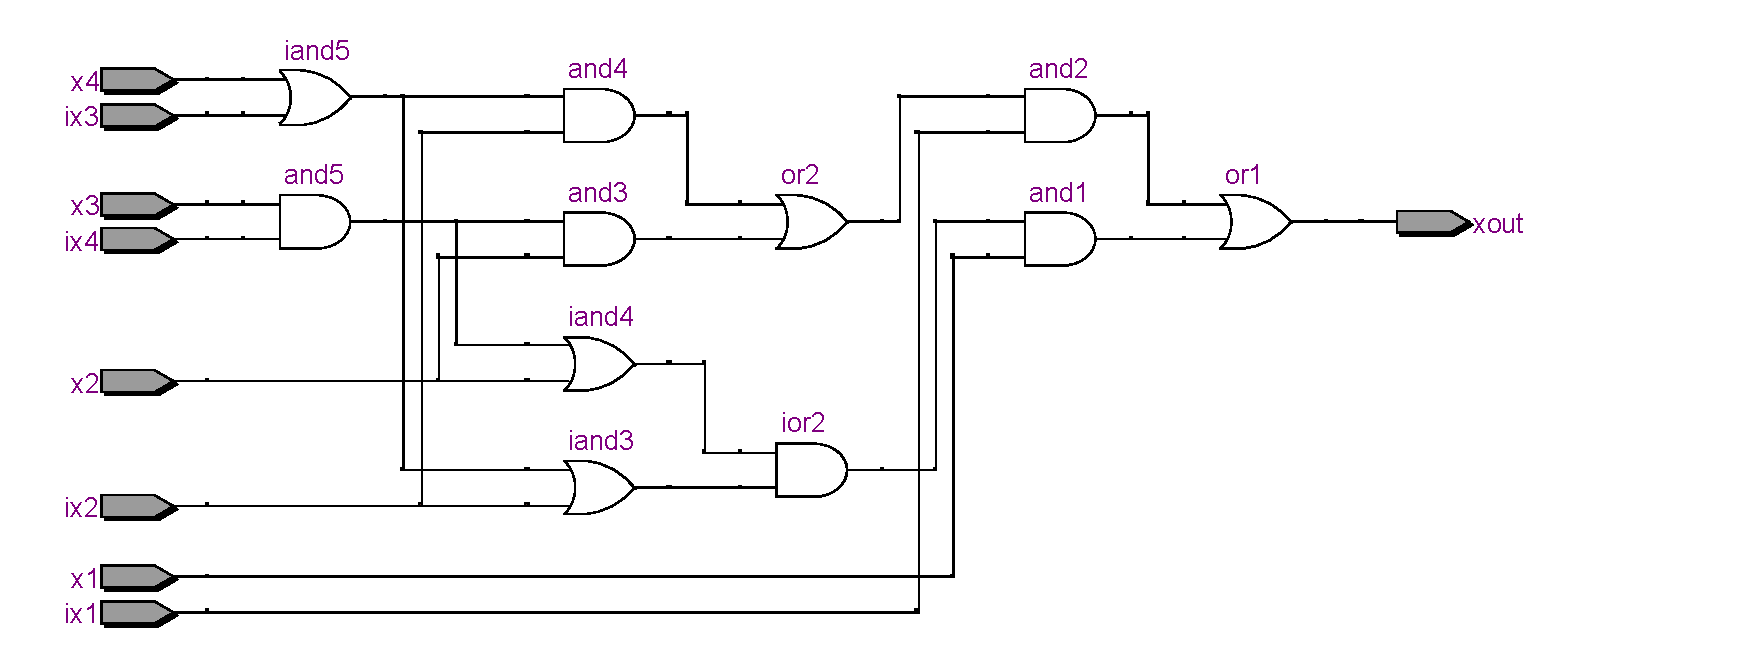
\includegraphics[scale=0.50]{images/endsk.pdf}

Am Ende konnten wir wieder 3 Gatter entfernen und konnten somit den Schaltkreis optimieren. Die neue Komplexit\"at ist nun $11$ und damit ist diese geringer als das Zweifache der Komplexit\"at des Urschaltkreises.


\end{document}